\documentclass[12pt,addpoints,answers]{repaso}
\grado{2}
\nivel{Secundaria}
\cicloescolar{2024-2025}
\materia{Matemáticas}
\unidad{1}
\title{Practica la Unidad}
\aprendizajes{
      \item Resuelve problemas de multiplicación y división con números enteros, fracciones y decimales positivos y negativos.
      \item Resuelve problemas de potencias con exponente entero y aproxima raíces cuadradas.
      \item Resuelve problemas que impliquen el uso de la notación científica.
      \item Calcula porcentajes de cantidades.
}
\author{Melchor Pinto, J.C.}
\begin{document}
\INFO
\begin{multicols}{2}
	\tableofcontents
\end{multicols}
\begin{questions}
	\addcontentsline{toc}{section}{Cálculos numéricos}
	\section*{Cálculos numéricos}

	\questionboxed[10]{Realiza las siguientes operaciones de \textit{cálculo numérico}:

		\begin{parts}
			\begin{multicols}{2}
				
\addcontentsline{toc}{subsection}{Suma de números}
	\subsection*{Suma de números}
				\part $849.332+242.25+469.381=$ \fillin[$1560.963$][0in]
				\part $27.05+34.99+0.1=$ \fillin[$62.14$][0in]
				\part $0.1+0.02+0.03+0.4=$ \fillin[$0.55$][0in]
				\part $0.11+2+3.8=$ \fillin[$5.91$][0in]
				
\addcontentsline{toc}{subsection}{Resta de números}
	\subsection*{Resta de números}
				\part $4934-451-682=$ \fillin[$3801$][0in]
				\part $0.1-0.02=$ \fillin[$0.08$][0in]
				\part $0.1-0.02-0.03-0.4=$ \fillin[$-0.35$][0in]
				\part $0.11-2-3.8=$ \fillin[$-5.69$][0in]
				
\addcontentsline{toc}{subsection}{Multiplicación de números}
	\subsection*{Multiplicación de números}
				\part $19.3\times6.27=$ \fillin[$121.011$][0in]
				\part $0.1\times0.02=$ \fillin[$0.002$][0in]
				\part $100.1\times 0.99=$ \fillin[$99.099$][0in]
				\part $0.11\times2\times3.8=$ \fillin[$0.836$][0in]
				
\addcontentsline{toc}{subsection}{División de números}
	\subsection*{División de números}
				\part $922\divisionsymbol1.2=$ \fillin[$768.333$][0in]
				\part $0.1\divisionsymbol0.02=$ \fillin[$5$][0in]
				\part $180\divisionsymbol 0.09=$ \fillin[$2000$][0in]
				\part $25.25\divisionsymbol 0.5=$ \fillin[$50.5$][0in]
				
\addcontentsline{toc}{subsection}{Resolución de problemas}
	\subsection*{Resolución de problemas}
				\part Entre José y su hermano están arreglando el jardín de su casa. José arregló $\dfrac{3}{8}$ del jardín y su hermano $\dfrac{1}{4}$. ¿Qué parte del jardín han arreglado?

				\begin{solutionbox}{3cm}
					\[\dfrac{3}{8}+\dfrac{1}{4}=\dfrac{3}{8}+\dfrac{2}{8}=\dfrac{5}{8}\]
				\end{solutionbox}
			\end{multicols}
		\end{parts}
	}

	\newpage

	\addcontentsline{toc}{section}{Números negativos}
	\section*{Números negativos}
	
\addcontentsline{toc}{subsection}{Ubicación en la recta numérica}
	\subsection*{Ubicación en la recta numérica}
	\questionboxed[4]{Escribe el número que representa el punto indicado en la recta numérica de cada uno de los siguientes incisos.

		\begin{multicols}{2}
			\begin{parts}
				\part 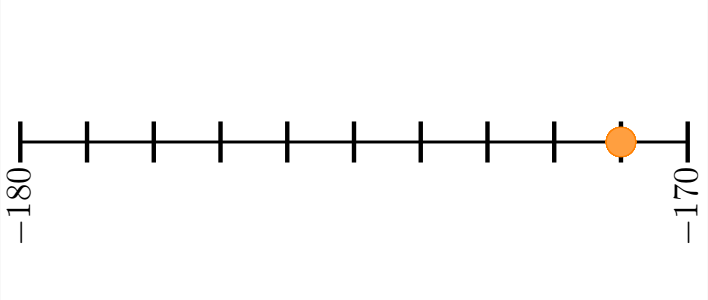
\includegraphics[width=140px]{../images/recta_num_-171.png} \\[-0.5em]   \fillin[$-171$][1.5in]
				\part 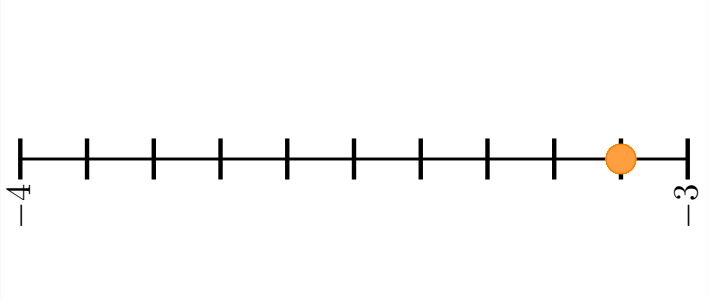
\includegraphics[width=140px]{../images/recta_num_-3.1.png} \\[-0.5em]   \fillin[$-3.1$][1.5in]
				\part 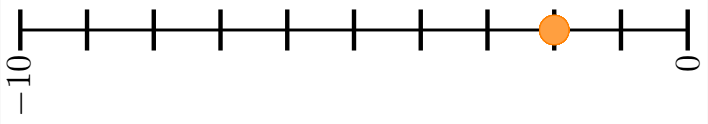
\includegraphics[width=140px]{../images/recta_num_-2.png}   \\[-0.5em] \fillin[$-2$][1.5in]
				\part 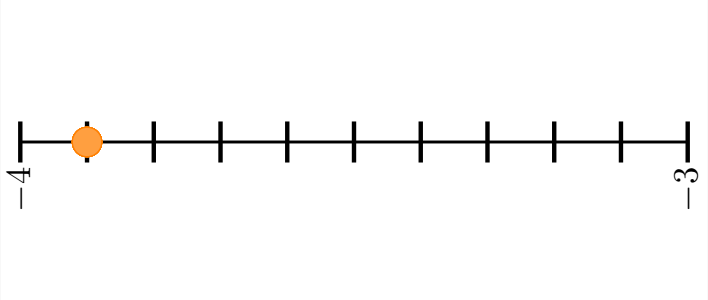
\includegraphics[width=140px]{../images/recta_num_-3.9.png} \\[-0.5em]   \fillin[$-3.9$][1.5in]
				\part 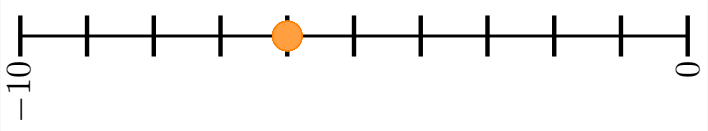
\includegraphics[width=140px]{../images/recta_num_-6.png}   \\[-0.5em] \fillin[$-6$][1.5in]
				\part 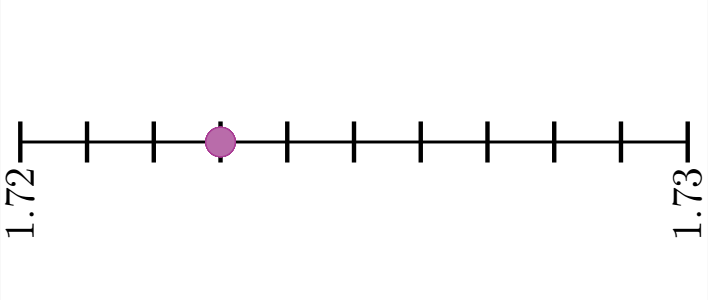
\includegraphics[width=140px]{../images/recta_num_1.723.png}\\[-0.5em]  \fillin[$1.723$][1.5in]
				\part 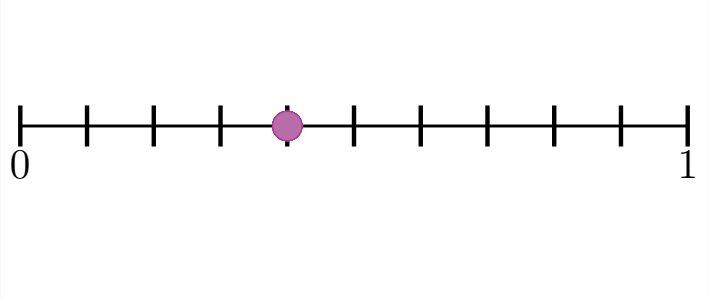
\includegraphics[width=140px]{../images/recta_num_0.4.png}  \\[-0.5em]  \fillin[$0.4.$][1.5in]
				\part 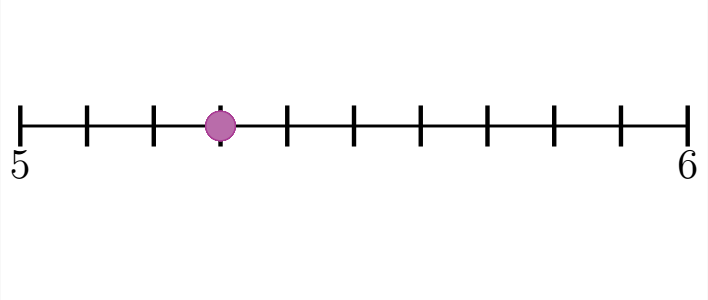
\includegraphics[width=140px]{../images/recta_num_5.3.png}  \\[-0.5em]  \fillin[$5.3.$][1.5in]
				\part 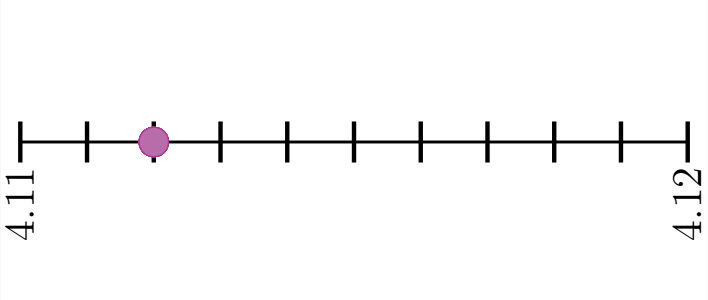
\includegraphics[width=140px]{../images/recta_num_4.112.png}\\[-0.5em]  \fillin[$4.11$][1.5in]
				\part 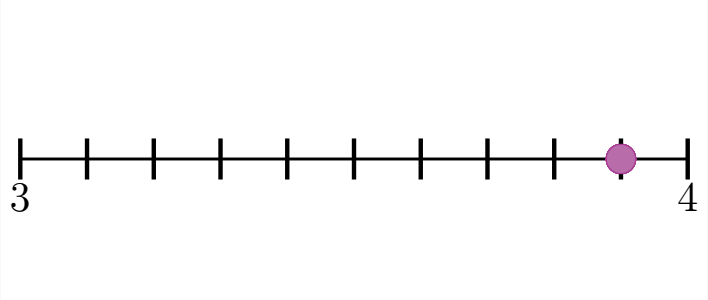
\includegraphics[width=140px]{../images/recta_num_3.9.png}  \\[-0.5em]  \fillin[$3.9.$][1.5in]
			\end{parts}
		\end{multicols}
	}

	
\addcontentsline{toc}{subsection}{Comparación de negativos}
	\subsection*{Comparación de negativos}
	\questionboxed[4]{Escribe sobre la línea el símbolo de mayor que ($>$), menor que ($<$), o igual ($=$) según corresponda.

		\begin{multicols}{2}
			\begin{parts}
				\part $-51$ \fillin[$>$][0.5in] $-55$\\[0.25em]
				% \part $-77$ \fillin[$>$][0.5in] $-177$\\[0.25em]
				\part $-100$ \fillin[$<$][0.5in] $-99$\\[0.25em]
				\part $-182$ \fillin[$>$][0.5in] $-189$\\[0.25em]
				\part $-97$ \fillin[$<$][0.5in] $-96.2$\\[0.25em]
				\part $-36$ \fillin[$>$][0.5in] $-39$\\[0.25em]
				\part $-3.5$ \fillin[$<$][0.5in] $-2.2$\\[0.25em]
				% \part $-12$ \fillin[$<$][0.5in] $-11$\\[0.25em]
				% \part $-10.001$ \fillin[$>$][0.5in] $-100.01$\\[0.25em]
				% \part $-0.99$ \fillin[$>$][0.5in] $1.01$
			\end{parts}
		\end{multicols}
	}


	
\addcontentsline{toc}{subsection}{Suma y resta con negativos}
	\subsection*{Suma y resta con negativos}
	\questionboxed[4]{Realiza las siguientes sumas y restas con números negativos:

		\begin{multicols}{2}
			\begin{parts}
				\part $-223+67=$ \fillin[$-156$][0in]
				\part $(16)-(-14)=$ \fillin[$30$][0in]
				\part $-(-15)-(-14)=$ \fillin[$-1$][0in]
				\part $-235+304=$ \fillin[$69$][0in]
				\part $198-189=$ \fillin[$9$][0in]
				\part $-201.1-9.4=$ \fillin[$-210.5$][0in]
				\part $201.1-9.4=$ \fillin[$191.7$][0in]
				\part $-201.1+9.4=$ \fillin[$-191.7$][0in]
			\end{parts}
		\end{multicols}
	}

	
\addcontentsline{toc}{subsection}{Multiplicación y división con negativos}
	\subsection*{Multiplicación y división con negativos}
	\questionboxed[4]{Realiza las siguientes multiplicaciones y divisiones con números negativos:
		\begin{multicols}{2}
			\begin{parts}
				\part $(31)\divisionsymbol (-62)=$ \fillin[$-\dfrac{1}{2}$][0in]
				\part $(-15)(-14)=$ \fillin[$210$][0in]
				\part $(-7)(20)=$ \fillin[$-140$][0in]
				\part $(50)\divisionsymbol (0.5)=$ \fillin[$100$][0in]
				\part $(-5)(-5)(-5)=$ \fillin[$-125$][0in]
				\part $(-220)\divisionsymbol (0.2)=$ \fillin[$-1100$][0in]
			\end{parts}
		\end{multicols}
	}

	
\addcontentsline{toc}{subsection}{Potencias con números negativos}
	\subsection*{Potencias con números negativos}
	\questionboxed[4]{Realiza las siguientes potencias de números negativos:
		\begin{multicols}{2}
			\begin{parts}
				\part $-7^2=$ \fillin[$-49$][0in]
				\part $(-5)^3=$ \fillin[$-125$][0in]
				\part $-2^4=$ \fillin[$-16$][0in]
				\part $(-3)^4=$ \fillin[$81$][0in]
				\part $-3^3=$ \fillin[$-27$][0in]
				\part $-(-2)^4=$ \fillin[$-16$][0in]
				\part $-(-3)^3=$ \fillin[$27$][0in]
				\part $(-2)^4=$ \fillin[$16$][0in]
			\end{parts}
		\end{multicols}
	}

	\addcontentsline{toc}{section}{Exponentes y notación científica}
	\section*{Exponentes y notación científica}
	\questionboxed[6]{Realiza las siguientes operaciones con exponentes:
		\begin{multicols}{3}
			\begin{parts}
				
\addcontentsline{toc}{subsection}{Suma de exponentes}
	\subsection*{Suma de exponentes}
				\part $(-5a^4)(-3a^2)=$ \fillin[$15a^6$][0in]
				\begin{solutionbox}{2cm}
					$(-5a^4)(-3a^2) = 15a^6$
				\end{solutionbox}

				\part $(-3a^4)(8a^2)=$
				\begin{solutionbox}{2cm}
					$(-3a^4)(8a^2) = -24a^6$
				\end{solutionbox}

				\part $4x^2\cdot x^5\cdot 5x^8=$
				\begin{solutionbox}{2cm}
					$4x^2\cdot x^5\cdot 5x^8 = 20x^{15}$
				\end{solutionbox}

				\part $x^2y^3z^4 \cdot x^5z^4=$
				\begin{solutionbox}{2cm}
					$x^2y^3z^4 \cdot x^5z^4 = x^7y^3z^8$
				\end{solutionbox}

				\columnbreak

				\part $x^3x^2x^3=$
				\begin{solutionbox}{2cm}
					$x^3x^2x^3 = x^8$
				\end{solutionbox}

				\part $7x^2\cdot 3x^4 \cdot 6x^2=$
				\begin{solutionbox}{2cm}
					$7x^2\cdot 3x^4 \cdot 6x^2 = 126x^8$
				\end{solutionbox}

				
\addcontentsline{toc}{subsection}{Resta de exponentes}
	\subsection*{Resta de exponentes}
				\part $\dfrac{x^{13}y^{18}z^{4}}{x^{11}y^{9}z^{4}}=$ \fillin[$x^2y^9$][0in]
				\begin{solutionbox}{2cm}
					$\dfrac{x^{13}y^{18}z^{4}}{x^{11}y^{9}z^{4}} = x^2y^9$
				\end{solutionbox}

				\part $\dfrac{x^{4}y^{12}z^{13}}{x^{3}y^{12}z^{13}}=$
				\begin{solutionbox}{2cm}
					$\dfrac{x^{4}y^{12}z^{13}}{x^{3}y^{12}z^{13}} = x$
				\end{solutionbox}

				\part $\dfrac{81a^5b^{12}c^9}{9a^3b^{7}c^5}=$
				\begin{solutionbox}{2cm}
					$\dfrac{81a^5b^{12}c^9}{9a^3b^{7}c^5} = 9a^2b^5c^4$
				\end{solutionbox}

				
\addcontentsline{toc}{subsection}{Multiplicación de exponentes}
	\subsection*{Multiplicación de exponentes}
				\part $(a^3b^2c^4)^3=$ \fillin[$a^9b^6c^{12}$][0in]
				\begin{solutionbox}{2cm}
					$(a^3b^2c^4)^3 = a^9b^6c^{12}$
				\end{solutionbox}

				\part $\left(x^4 y^5\right)^6=$
				\begin{solutionbox}{2cm}
					$\left(x^4 y^5\right)^6 = x^{24}y^{30}$
				\end{solutionbox}

				\part $\left(a^3 b^5 c^{11} \right)^7=$
				\begin{solutionbox}{2cm}
					$\left(a^3 b^5 c^{11} \right)^7 = a^{21}b^{35}c^{77}$
				\end{solutionbox}
			\end{parts}
		\end{multicols}
	}

	\newpage
	
\addcontentsline{toc}{subsection}{Notación científica}
	\subsection*{Notación científica}
	\questionboxed[4]{Escribe en notación científica los siguientes números:
		\begin{multicols}{2}
			\begin{parts}
				\part $50500=$ \fillin[$5.05 \cdot 10^4$][1.5in]
				\part $0.00000000024=$ \fillin[$2.4 \cdot 10^{-10}$][1.5in]
				\part $101=$ \fillin[$1.01 \cdot 10^2$][1.5in]
				\part $750000000000=$ \fillin[$7.5 \cdot 10^{11}$][1.5in]
				\part $80008000=$ \fillin[$8.0008 \cdot 10^7$][1.5in]
				\part $0.003=$ \fillin[$3 \cdot 10^{-3}$][1.5in]
				\part $0.0000204=$ \fillin[$2.04 \cdot 10^{-5}$][1.5in]
				\part $0.0000000000099=$ \fillin[$9.9 \cdot 10^{-12}$][1.5in]
				\part $606000000000000000=$ \fillin[$6.06 \cdot 10^{17}$][1.5in]
				\part $102100000000000=$ \fillin[$1.021 \cdot 10^{14}$][1.5in]
			\end{parts}
		\end{multicols}
	}

	\questionboxed[4]{Escribe en notación decimal los siguientes números:
		\begin{multicols}{2}
			\begin{parts}
				\part $1.2 \cdot 10^3=$ \fillin[$1200$][1.5in]
				\part $2.3 \cdot 10^2=$ \fillin[$230$][1.5in]
				\part $4 \cdot 10^{-3}=$ \fillin[$0.004$][1.5in]
				\part $7 \cdot 10^{-6}=$ \fillin[$0.000007$][1.5in]
				\part $2 \cdot 10^6=$ \fillin[$2000000$][1.5in]
				\part $-3 \cdot 10^{-4}=$ \fillin[$-0.0003$][1.5in]
				\part $1.2 \cdot 10^{-1}=$ \fillin[$0.12$][1.5in]
				\part $80.3 \cdot 10^{-2}=$ \fillin[$0.803$][1.5in]
				\part $3 \cdot 10^{-3}=$ \fillin[$0.003$][1.5in]
				\part $3 \cdot 10^{8}=$ \fillin[$300000000$][1.5in]
			\end{parts}
		\end{multicols}
	}

	\addcontentsline{toc}{section}{Plano cartesiano y la recta}
	\section*{Plano cartesiano y la recta}
	\questionboxed[10]{Escribe las coordenadas de los puntos indicados en el plano cartesiano de cada uno de los siguientes incisos.
		\begin{multicols}{2}
			\begin{parts}
				
\addcontentsline{toc}{subsection}{}
	\subsection*{Ubicación en el plano cartesiano}
				\part Coordenadas del punto A = \fillin[$(1,5)$][0in]
				\part Coordenadas del punto B = \fillin[$(-3,6)$][0in]
				\part Coordenadas del punto C = \fillin[$(5,-3)$][0in]
				\part Coordenadas del punto D = \fillin[$(-5,0$][0in]
				\part Coordenadas del punto E = \fillin[$(0,-7)$][0in]
				
\addcontentsline{toc}{subsection}{}
	\subsection*{Cuadrantes en el plano cartesiano}
				\part el punto C en el plano cartesiano: \fillin[4 cuad.][1in]
				\part el punto B en el plano cartesiano: \fillin[2 cuad.][1in]
				\part el punto A en el plano cartesiano: \fillin[1 cuad.][1in]
			\end{parts}
			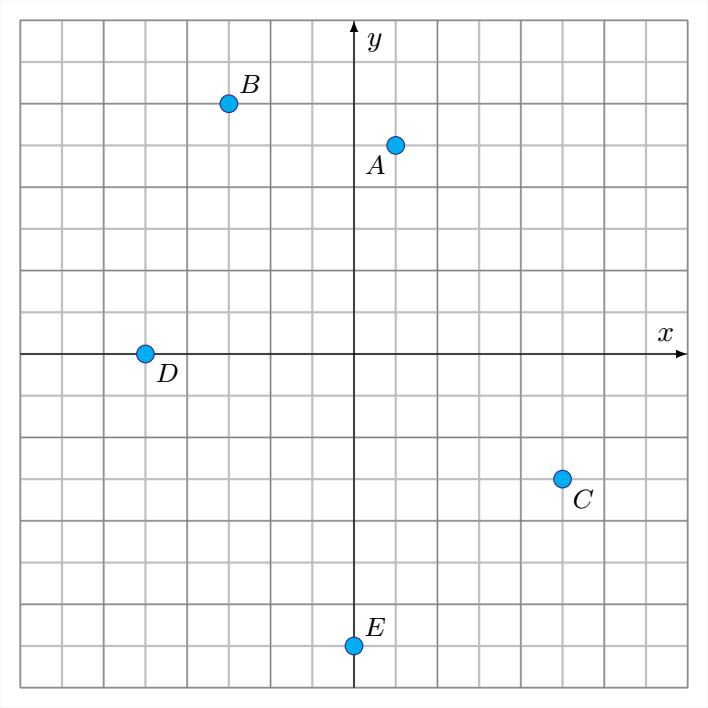
\includegraphics[width=0.8\linewidth]{../images/imagen_plano01.png}
		\end{multicols}
	}


	\newpage
	
\addcontentsline{toc}{subsection}{Pendiente de una recta}
	\subsection*{Pendiente de una recta}
	\questionboxed[8]{Selecciona la opcion que corresponde a la pendiente de la recta en cada uno de los siguientes incisos:
		\begin{multicols}{2}
			\begin{parts}
				\part
				\begin{minipage}{0.6\linewidth}
					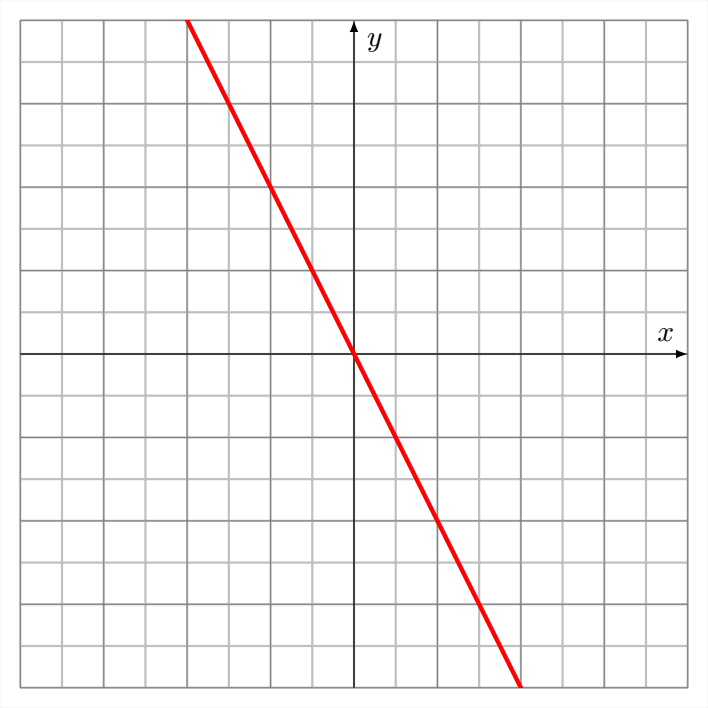
\includegraphics[width=\linewidth]{../images/plano_cart_rect_-2x.png}
				\end{minipage}%
				\begin{minipage}{0.5\linewidth}
					\begin{choices}
						\choice Positiva
						\CorrectChoice Negativa
						\choice Cero
						\choice Indefinida
					\end{choices}
				\end{minipage}

				\part
				\begin{minipage}{0.6\linewidth}
					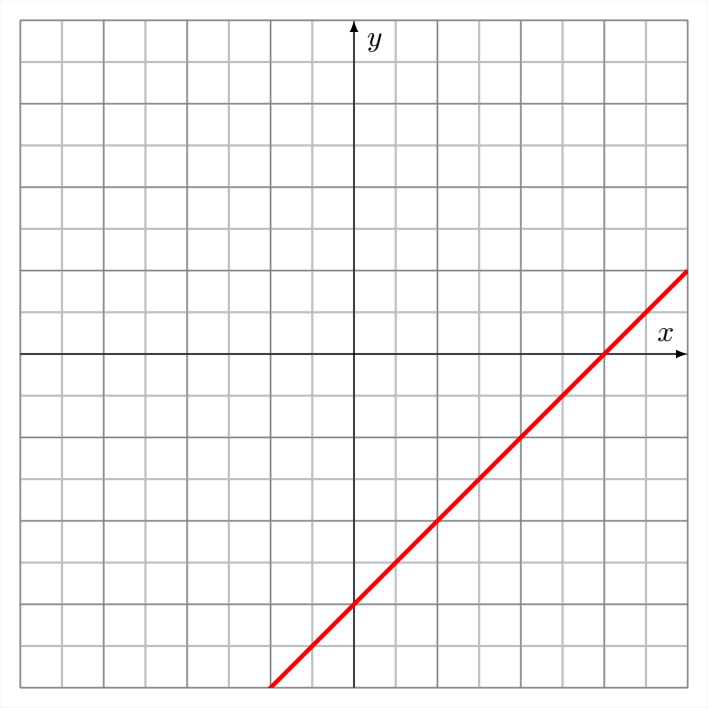
\includegraphics[width=\linewidth]{../images/plano_cart_rect_x-6.png}
				\end{minipage}%
				\begin{minipage}{0.5\linewidth}
					\begin{choices}
						\CorrectChoice Positiva
						\choice Negativa
						\choice Cero
						\choice Indefinida
					\end{choices}
				\end{minipage}

				\part
				\begin{minipage}{0.6\linewidth}
					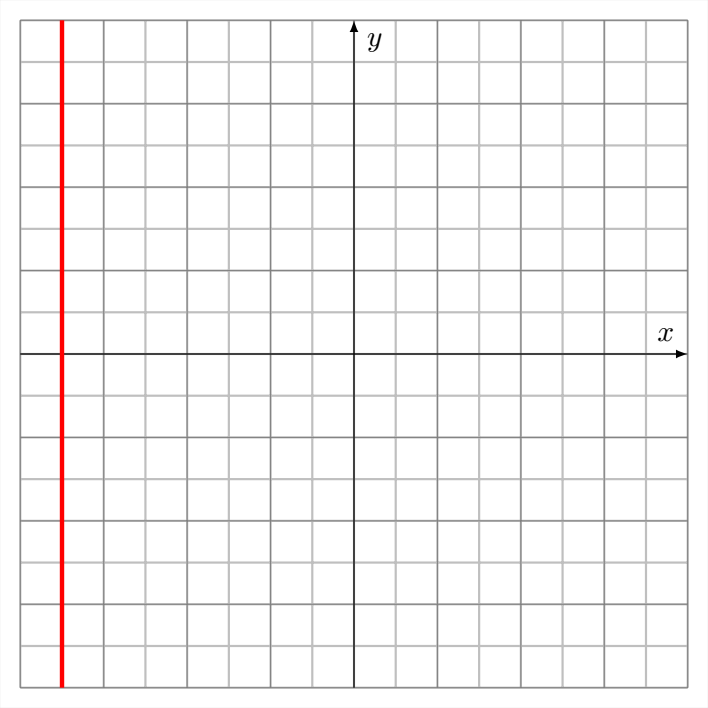
\includegraphics[width=\linewidth]{../images/plano_cart_rect_inf.png}
				\end{minipage}%
				\begin{minipage}{0.5\linewidth}
					\begin{choices}
						\choice Positiva
						\choice Negativa
						\choice Cero
						\CorrectChoice Indefinida
					\end{choices}
				\end{minipage}

				\part
				\begin{minipage}{0.6\linewidth}
					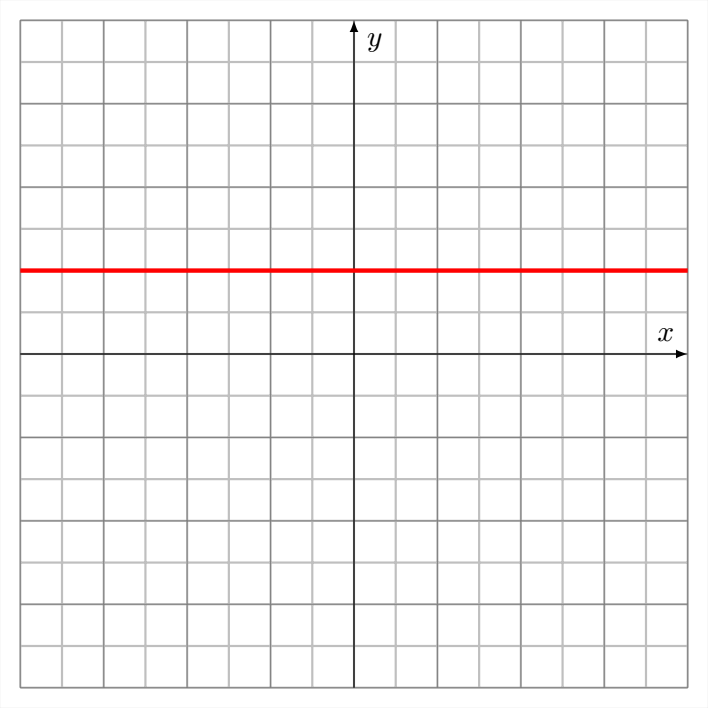
\includegraphics[width=\linewidth]{../images/plano_cart_rect_0.png}
				\end{minipage}%
				\begin{minipage}{0.5\linewidth}
					\begin{choices}
						\choice Positiva
						\choice Negativa
						\CorrectChoice Cero
						\choice Indefinida
					\end{choices}
				\end{minipage}
			\end{parts}
		\end{multicols}
	}

	
\addcontentsline{toc}{subsection}{Pendiente y ordenada}
	\subsection*{Pendiente y ordenada}
	\questionboxed[8]{Identifica la pendiente y ordenada de las siguientes rectas:
		\begin{multicols}{3}
			\begin{parts}
				\part $y=-2x$ \\[1em]
				Pendiente = \fillin[$-2$][0in]\\[0.5em]
				Ordenada = \fillin[$0$][0in]

				\part $y=-\dfrac{2}{3}x-5$ \\[1em]
				Pendiente = \fillin[$-\dfrac{2}{3}$][0in]\\[0.5em]
				Ordenada = \fillin[$-5$][0in]

				\part $y=3x+2$ \\[1em]
				Pendiente = \fillin[$3$][0in]\\[0.5em]
				Ordenada = \fillin[$2$][0in]

				\part $y=\dfrac{1}{2}x-3$ \\[1em]
				Pendiente = \fillin[$\dfrac{1}{2}$][0in]\\[0.5em]
				Ordenada = \fillin[$-3$][0in]

				\part $y=-\dfrac{1}{2}x+3$ \\[1em]
				Pendiente = \fillin[$-\dfrac{1}{2}$][0in]\\[0.5em]
				Ordenada = \fillin[$3$][0in]

				\part $y=-3x+3$ \\[1em]
				Pendiente = \fillin[$-3$][0in]\\[0.5em]
				Ordenada = \fillin[$3$][0in]
			\end{parts}
		\end{multicols}
	}

	\newpage
	
\addcontentsline{toc}{subsection}{Ecuación de una recta}
	\subsection*{Ecuación de una recta}
	\questionboxed[4]{Escribe la ecuación de cada una de las rectas en los siguientes planos cartesianos:
		\begin{multicols}{2}
			\begin{parts}
				\part
				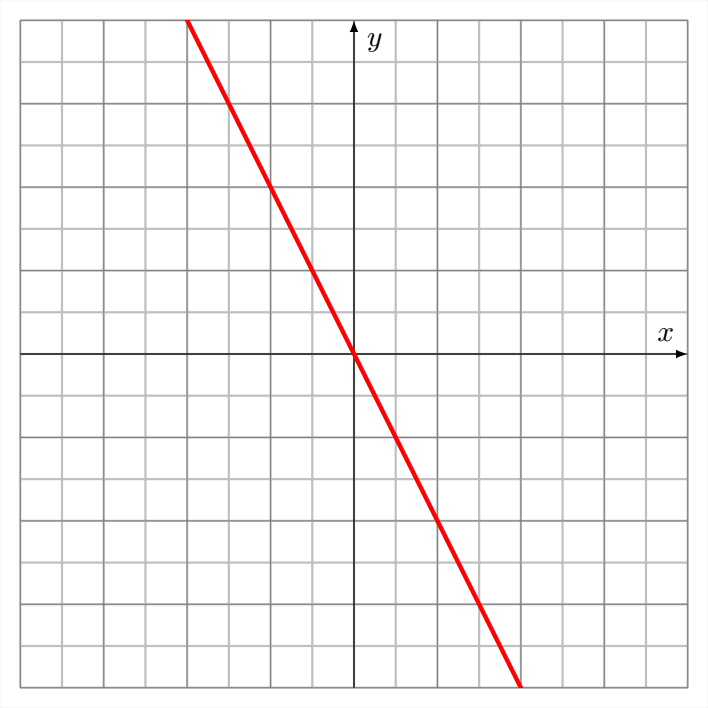
\includegraphics[width=.8\linewidth]{../images/plano_cart_rect_-2x.png}\\
				\fillin[$y=-2x$][2in]

				\part
				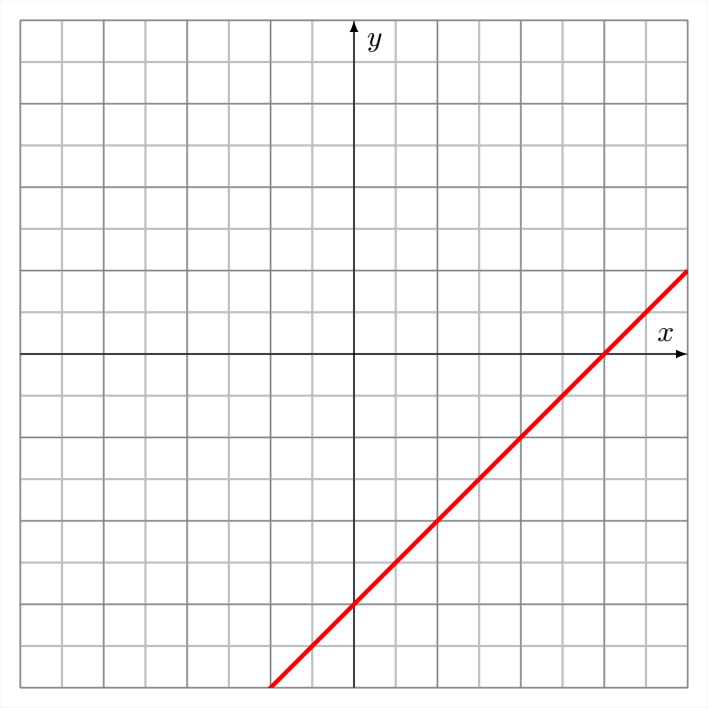
\includegraphics[width=.8\linewidth]{../images/plano_cart_rect_x-6.png}\\
				\fillin[$y=x-6$][2in]
			\end{parts}
		\end{multicols}
	}

	\addcontentsline{toc}{section}{Porcentajes}
	\section*{Porcentajes}
	
\addcontentsline{toc}{subsection}{Porcentajes a decimal}
	\subsection*{Porcentajes a decimal}

	\questionboxed[4]{Escribe el número decimal que representa cada porcentaje:

		\begin{multicols}{2}
			\begin{parts}
				\part Convierte 401\% a un número decimal. \fillin[$4.01$][0in]
				\part Convierte 6\% a un número decimal. \fillin[$0.06$][0in]
				\part Convierte 0.5\% a un número decimal. \fillin[$0.005$][0in]
				\part Convierte 150\% a un número decimal. \fillin[$1.5$][0in]
				\part Convierte 33\% a un número decimal. \fillin[$0.33$][0in]
				\part Convierte 20.9\% a un número decimal. \fillin[$0.209$][0in]
			\end{parts}
		\end{multicols}
	}

	
\addcontentsline{toc}{subsection}{Decimal a porcentaje}
	\subsection*{Decimal a porcentaje}
	\questionboxed[4]{Escribe el porcentaje que representa cada número decimal:

		\begin{multicols}{2}
			\begin{parts}
				\part Expresa 1.44 como un porcentaje. \fillin[$144\%$][0in]
				\part Expresa 0.092 como un porcentaje. \fillin[$9.2\%$][0in]
				\part Expresa 0.0005 como un porcentaje. \fillin[$0.05\%$][0in]
				\part Expresa 5.5 como un porcentaje. \fillin[$550\%$][0in]
				\part Expresa 0.33 como un porcentaje. \fillin[$33\%$][0in]
				\part Expresa 0.209 como un porcentaje. \fillin[$20.9\%$][0in]
			\end{parts}
		\end{multicols}
	}

	
\addcontentsline{toc}{subsection}{Porcentaje de cantidades}
	\subsection*{Porcentaje de cantidades}
	\questionboxed[8]{Calcula los porcentajes de cada una de las siguientes cantidades:
		\begin{multicols}{2}
			\begin{parts}
				\part ¿Cuál es el 225\% de 600?
				\begin{solutionbox}{1.5cm}
					\[\dfrac{600\times 225\%}{100\%}=1350\]
				\end{solutionbox}

				\part Si se sabe que 30 es el 6\% de cierta cantidad, ¿cuál es esta cantidad?
				\begin{solutionbox}{1.5cm}
					\[\dfrac{30\times 100\%}{6\%}=500\]
				\end{solutionbox}

				\part ¿Cuál es el 23\% de 59?
				\begin{solutionbox}{1.5cm}
					\[\dfrac{59\times 23\%}{100\%}=13.57\]
				\end{solutionbox}

				\part Si se sabe que 40 es el 250\% de cierta cantidad, ¿cuál es esta cantidad?
				\begin{solutionbox}{1.5cm}
					\[\dfrac{40\times 100\%}{250\%}=16\]
				\end{solutionbox}
			\end{parts}
		\end{multicols}
	}
	
\addcontentsline{toc}{subsection}{Resolución de problemas}
	\subsection*{Resolución de problemas}
	\questionboxed[10]{Resuelve los siguientes problemas:
		\begin{parts}
			\part El costo de una camisa es de \$800 pesos, si se les hace un descuento del 20\%, ¿cuánto pagaré en total por la camisa?
			\begin{solutionbox}{2cm}
				\[\$800\times 20\%=\$160\]
				\[\$800-\$160=\$640\]
			\end{solutionbox}

			\part El 24\% de los habitantes de un pueblo tienen menos de 30 años. ¿Cuántos habitantes tiene el pueblo si hay 120 jóvenes menores de 30 años?
			\begin{solutionbox}{2cm}
				\[\dfrac{120\times 100\%}{24\%}=500\]
			\end{solutionbox}
		\end{parts}
	}
\end{questions}
\end{document}